\chapter{Тригонометрия}
\begin{definition}\term{Радиан} (\emph{radian}) — единица измерения угла. Угол в \(1\) радиан — центральный угол, которому соответствует дуга длины, равной радиусу окружности. Радианная мера центрального угла равна \(\alpha=\frac{l}{r}\), где \(l\) — длина дуги, \(r>0\) — радиус. Полный оборот: \(2\pi\) радиан, то есть \(360^\circ\).\end{definition}
Положительные углы отсчитывают от точки \((1;0)\) единичной окружности против часовой стрелки, отрицательные — по часовой.
\begin{definition}\term{Косинус} (\emph{cosine}) \(\cos\alpha\) — горизонтальная координата точки единичной окружности, полученной поворотом точки \((1;0)\) на угол \(\alpha\).\end{definition}
\begin{definition}\term{Синус} (\emph{sine}) \(\sin\alpha\) — вертикальная координата точки единичной окружности, полученной поворотом точки \((1;0)\) на угол \(\alpha\).\end{definition}
\begin{definition}\term{Тангенс} (\emph{tangent}): \(\tan  \alpha  = \frac{\sin  \alpha }{\cos  \alpha }\) при \(\cos  \alpha  \ne  0\).\end{definition}
\begin{definition}\term{Период функции} (\emph{period of a function}) — ненулевое число \(T\), при сдвиге аргумента на которое область определения сохраняется и \(f (x + T) = f (x)\).\end{definition}
\section*{Основные тождества и свойства}
\(\sin ^{2} \alpha  + \cos ^{2} \alpha  = 1\). Значения синуса и косинуса лежат в \([- 1;\allowbreak 1]\).\par
\(\sin  (- \alpha ) = - \sin  \alpha ;\allowbreak \cos  (- \alpha ) = \cos  \alpha \).\par
\(\sin  (\pi  - \alpha ) = \sin  \alpha ;\allowbreak \cos  (\pi  - \alpha ) = - \cos  \alpha \).\par
Наименьший положительный период синуса и косинуса равен \(2 \pi \). Для \(\sin  (kx)\) и \(\cos  (kx)\) при \(k \ne  0\) он равен \(\frac{2 \pi }{| k |}\).\par
\section*{Прямоугольный треугольник}
Для острого угла синус — \(\frac{\text{противолежащий катет}}{\text{гипотенуза}}\); косинус — \(\frac{\text{прилежащий катет}}{\text{гипотенуза}}\); тангенс — \(\frac{\text{противолежащий катет}}{\text{прилежащий катет}}\).\par
\section*{Значения, которые стоит знать}
\(\sin  0 = 0;\allowbreak \sin  (\frac{\pi }{6}) = \frac{1}{2};\allowbreak \sin  (\frac{\pi }{4}) = \frac{\sqrt{2}}{2};\allowbreak \sin  (\frac{\pi }{3}) = \frac{\sqrt{3}}{2};\allowbreak \sin  (\frac{\pi }{2}) = 1\).\par
\(\cos  0 = 1;\allowbreak \cos  (\frac{\pi }{6}) = \frac{\sqrt{3}}{2};\allowbreak \cos  (\frac{\pi }{4}) = \frac{\sqrt{2}}{2};\allowbreak \cos  (\frac{\pi }{3}) = \frac{1}{2};\allowbreak \cos  (\frac{\pi }{2}) = 0\).\par
{\small\textit{Пример: \(60 {}^{\circ} = \frac{\pi }{3}\) радиан, потому что \(60 \cdot  \frac{\pi }{180} = \frac{\pi }{3}\).}}\par

\section*{Обратные тригонометрические функции}
На всей числовой прямой синус и косинус принимают одни и те же значения много раз. Чтобы получить обратную функцию, нужно выбрать промежуток, на котором каждому значению соответствует ровно один аргумент.
\begin{definition}\term{Арксинус} (arcsine) \(\arcsin t\) — единственный угол \(\alpha\in[-\frac\pi2;\frac\pi2]\), для которого \(\sin\alpha=t\). Область определения: \(t\in[-1;1]\); область значений: \([-\frac\pi2;\frac\pi2]\).\end{definition}
\begin{definition}\term{Арккосинус} (arccosine) \(\arccos t\) — единственный угол \(\alpha\in[0;\pi]\), для которого \(\cos\alpha=t\). Область определения: \(t\in[-1;1]\); область значений: \([0;\pi]\).\end{definition}
\begin{definition}\term{Арктангенс} (arctangent) \(\arctan t\) — единственный угол \(\alpha\in(-\frac\pi2;\frac\pi2)\), для которого \(\tan\alpha=t\). Область определения: \(t\in\mathbb R\); область значений: \((-\frac\pi2;\frac\pi2)\).\end{definition}
Синус на \([-\frac\pi2;\frac\pi2]\) и тангенс на \((-\frac\pi2;\frac\pi2)\) строго возрастают, а косинус на \([0;\pi]\) строго убывает. Именно эти ограничения позволяют определить обратные функции. Их графики получают отражением соответствующих ограниченных графиков относительно \(y=x\).
По определениям \(\sin(\arcsin t)=t\), \(\cos(\arccos t)=t\) при \(t\in[-1;1]\), а \(\tan(\arctan t)=t\) при всех действительных \(t\). Обратный порядок требует ограничения аргумента: \(\arcsin(\sin x)=x\) только при \(x\in[-\frac\pi2;\frac\pi2]\); \(\arccos(\cos x)=x\) только при \(x\in[0;\pi]\); \(\arctan(\tan x)=x\) только при \(x\in(-\frac\pi2;\frac\pi2)\). Вне этих промежутков результат нужно привести к области значений обратной функции. В частности, \(\arcsin(\sin\frac{5\pi}6)=\arcsin\frac12=\frac\pi6\), а не \(\frac{5\pi}6\). При \(x=\frac\pi2+\pi k\), \(k\in\mathbb Z\), сама запись \(\arctan(\tan x)\) не определена.
\begin{theorem}[Связь арксинуса и арккосинуса]
Для любого \(t\in[-1;1]\) выполнено \(\arcsin t+\arccos t=\frac\pi2\).
\end{theorem}
\begin{proof}
Пусть \(\alpha=\arcsin t\); тогда \(\alpha\in[-\frac\pi2;\frac\pi2]\) и \(\sin\alpha=t\). Угол \(\beta=\frac\pi2-\alpha\) принадлежит \([0;\pi]\), а \(\cos\beta=\sin\alpha=t\). По единственности угла в определении арккосинуса \(\beta=\arccos t\), откуда следует нужное равенство.
\end{proof}
В некоторых источниках обозначения \(\sin^{-1}t\), \(\cos^{-1}t\), \(\tan^{-1}t\) означают обратные функции. Чтобы не путать их с обратными числами \(\frac1{\sin t}\), \(\frac1{\cos t}\), \(\frac1{\tan t}\), здесь используем только записи \(\arcsin\), \(\arccos\), \(\arctan\).

\clearpage\section*{Графики}
\begin{center}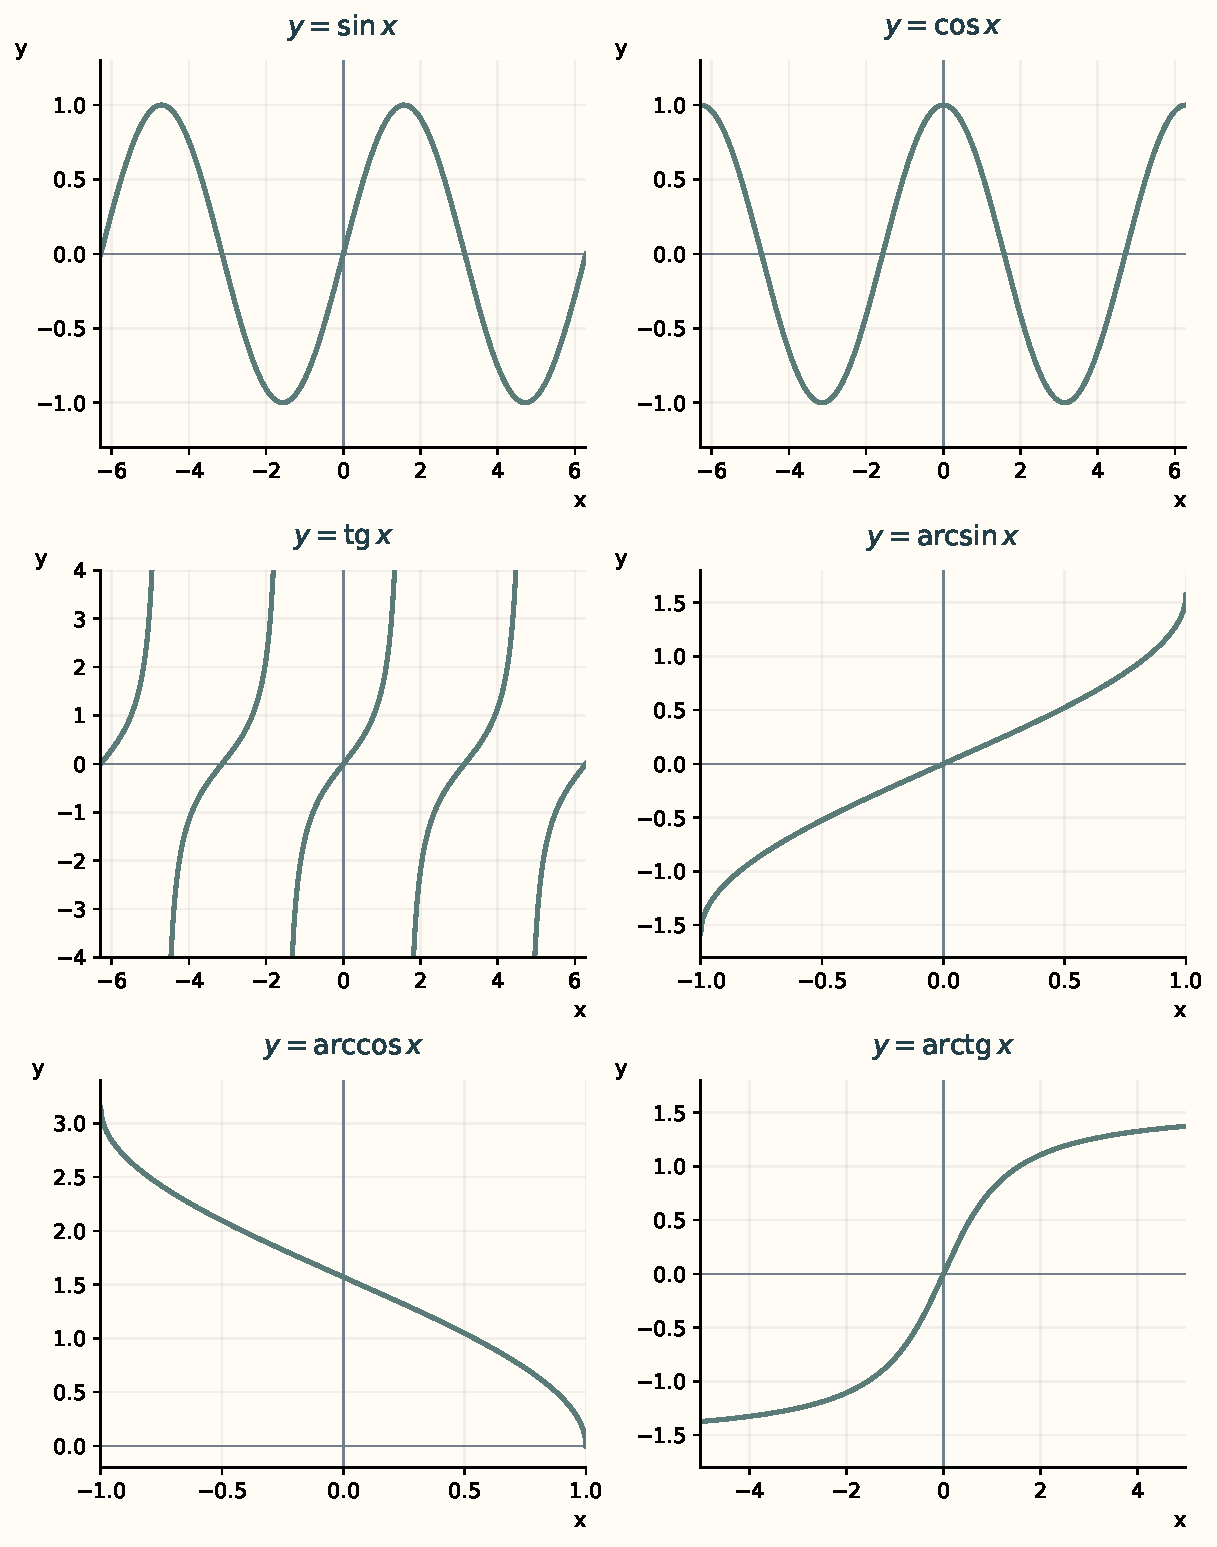
\includegraphics[width=\textwidth,height=.79\textheight,keepaspectratio]{images/atlas-trigonometry.pdf}\par\small Тригонометрические и обратные функции\end{center}
\Needspace{7\baselineskip}\section*{Задачи}
\begin{enumerate}[label={},leftmargin=3.2em,itemsep=10pt]
\Needspace{3\baselineskip}\item[\textbf{15.1.}] Переведи \(30 {}^{\circ},\allowbreak 90 {}^{\circ}\) и \(150 {}^{\circ}\) в радианы.
\Needspace{3\baselineskip}\item[\textbf{15.2.}] Переведи \(\frac{\pi }{4}\) и \(\frac{7 \pi }{6}\) в градусы.
\Needspace{3\baselineskip}\item[\textbf{15.3.}] Вычисли \(\sin  (\frac{\pi }{6}),\allowbreak \cos  (\frac{\pi }{3}),\allowbreak \tan  (\frac{\pi }{4})\).
\Needspace{3\baselineskip}\item[\textbf{15.4.}] Определи знаки \(\sin \) и \(\cos \) для угла \(\frac{5 \pi }{6}\).
\Needspace{3\baselineskip}\item[\textbf{15.5.}] Найди \(\sin  (- \frac{\pi }{6})\) и \(\cos  (- \frac{\pi }{3})\).
\Needspace{3\baselineskip}\item[\textbf{15.6.}] Упрости \(\sin ^{2} x + \cos ^{2} x + 2\).
\Needspace{3\baselineskip}\item[\textbf{15.7.}] Если \(\sin  x = \frac{3}{5}\) и \(0 < x < \frac{\pi }{2}\), найди \(\cos  x\) и \(\tan  x\).
\Needspace{3\baselineskip}\item[\textbf{15.8.}] Найди \(\sin  (\pi  - x)\) и \(\cos  (\pi  - x)\) через функции \(x\).
\Needspace{3\baselineskip}\item[\textbf{15.9.}] Реши \(\sin  x = 0\) при \(x \in  [0;\allowbreak 2 \pi ]\).
\Needspace{3\baselineskip}\item[\textbf{15.10.}] Реши \(\cos  x = \frac{1}{2}\) при \(x \in  [0;\allowbreak 2 \pi ]\).
\Needspace{3\baselineskip}\item[\textbf{15.11.}] Построй \(y = \sin  x\) на \([0;\allowbreak 2 \pi ]\). Укажи нули, максимум и минимум.
\Needspace{3\baselineskip}\item[\textbf{15.12.}] Найди наименьший положительный период \(y = \sin  (2 x)\).
\Needspace{3\baselineskip}\item[\textbf{15.13.}] Из жизни. Солнечный луч образует с землёй угол \(45 {}^{\circ}\). Тень вертикального столба равна \(6\) м. Найди высоту столба.
\Needspace{3\baselineskip}\item[\textbf{15.14.}] Из жизни. Лестница длиной \(10\) м образует с горизонтальной землёй угол \(30 {}^{\circ}\). На какой высоте находится её верх?
\Needspace{3\baselineskip}\item[\textbf{15.15.}] Из жизни. Колесо обозрения радиусом \(10\) м имеет центр на высоте \(12\) м. Высота кабинки \(h = 12 + 10 \sin  \alpha \). Найди высоту при \(\alpha  = 0,\allowbreak \frac{\pi }{2}\) и \(\frac{3 \pi }{2}\).
\Needspace{3\baselineskip}\item[\textbf{15.16.}\starmark] Реши \(2 \sin ^{2} x - 3 \sin  x + 1 = 0\) при \(x \in  [0;\allowbreak 2 \pi ]\).
\Needspace{3\baselineskip}\item[\textbf{15.17.}\starmark] Луч образует с землёй угол \(30 {}^{\circ}\). Длина тени вертикального дерева \(12\) м. Найди высоту дерева в точном виде.
\Needspace{3\baselineskip}\item[\textbf{15.18.}\starmark] Высота кабинки задана \(h (t) = 15 - 12 \cos  (\frac{\pi  t}{20})\) метров, где \(t\) — секунды от начала движения. Найди минимальную и максимальную высоты и время первого достижения максимума при \(t \ge  0\).
\begin{center}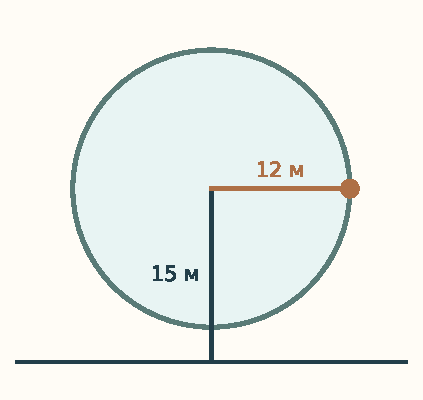
\includegraphics[width=.7\linewidth,height=45mm,keepaspectratio]{images/diagram-wheel.pdf}\end{center}
\Needspace{3\baselineskip}\item[\textbf{15.19.}\starmark] Докажи нечётность арксинуса: \(\arcsin(-t)=-\arcsin t\) для \(t\in[-1;1]\). В доказательстве проверь область значений угла, а не только равенство синусов.
\Needspace{3\baselineskip}\item[\textbf{15.20.}\starmark] Докажи тождество \(\arccos(-t)=\pi-\arccos t\) при \(t\in[-1;1]\).
\Needspace{3\baselineskip}\item[\textbf{15.21.}] Вычисли \(\arcsin0\), \(\arcsin\frac12\), \(\arcsin(-\frac{\sqrt3}{2})\).
\Needspace{3\baselineskip}\item[\textbf{15.22.}] Вычисли \(\arccos(-\frac12)\), \(\arccos1\), \(\arccos0\).
\Needspace{3\baselineskip}\item[\textbf{15.23.}] Вычисли \(\arctan(-1)\), \(\arctan\sqrt3\), \(\arctan0\).
\Needspace{3\baselineskip}\item[\textbf{15.24.}\starmark] Вычисли \(\arcsin(\sin\frac{5\pi}6)\), \(\arccos(\cos\frac{5\pi}3)\), \(\arctan(\tan\frac{3\pi}4)\). Для каждого ответа проверь диапазон обратной функции.
\Needspace{3\baselineskip}\item[\textbf{15.25.}] Найди \(\cos(\arcsin\frac35)\) и \(\sin(\arccos(-\frac35))\). Обоснуй выбор знака квадратного корня.
\Needspace{3\baselineskip}\item[\textbf{15.26.}] Реши \(\arcsin(2x-1)=\frac\pi6\). Сначала найди область допустимых значений.
\Needspace{3\baselineskip}\item[\textbf{15.27.}] Реши \(\arctan(x-2)=-\frac\pi4\).
\Needspace{3\baselineskip}\item[\textbf{15.28.}] Построй эскиз \(y=\arctan x\), отметив точки с аргументами \(-1\), \(0\), \(1\). Укажи область определения, область значений и чётность. Может ли значение функции быть равным \(\frac\pi2\)?
\end{enumerate}
